\chapter{System Design}

\section{System Architecture}
OpenArmor's architecture is designed to integrate and enhance the capabilities of Wazuh, OSquery, and Sysmon while introducing innovative features like eBPF logging and AI-driven analysis. The high-level architecture consists of the following components:

\begin{itemize}
    \item OpenArmor Core: Central management and analysis engine
    \item Agent Network: Distributed agents for data collection (including Wazuh agents)
    \item eBPF Engine: Kernel-level data collection and processing
    \item AI Analytics Module: Machine learning-based threat detection and analysis
    \item OCSF Normalization Layer: Log standardization and interoperability
    \item Web Dashboard: User interface for monitoring and management
\end{itemize}

\begin{figure}[h]
    \centering
    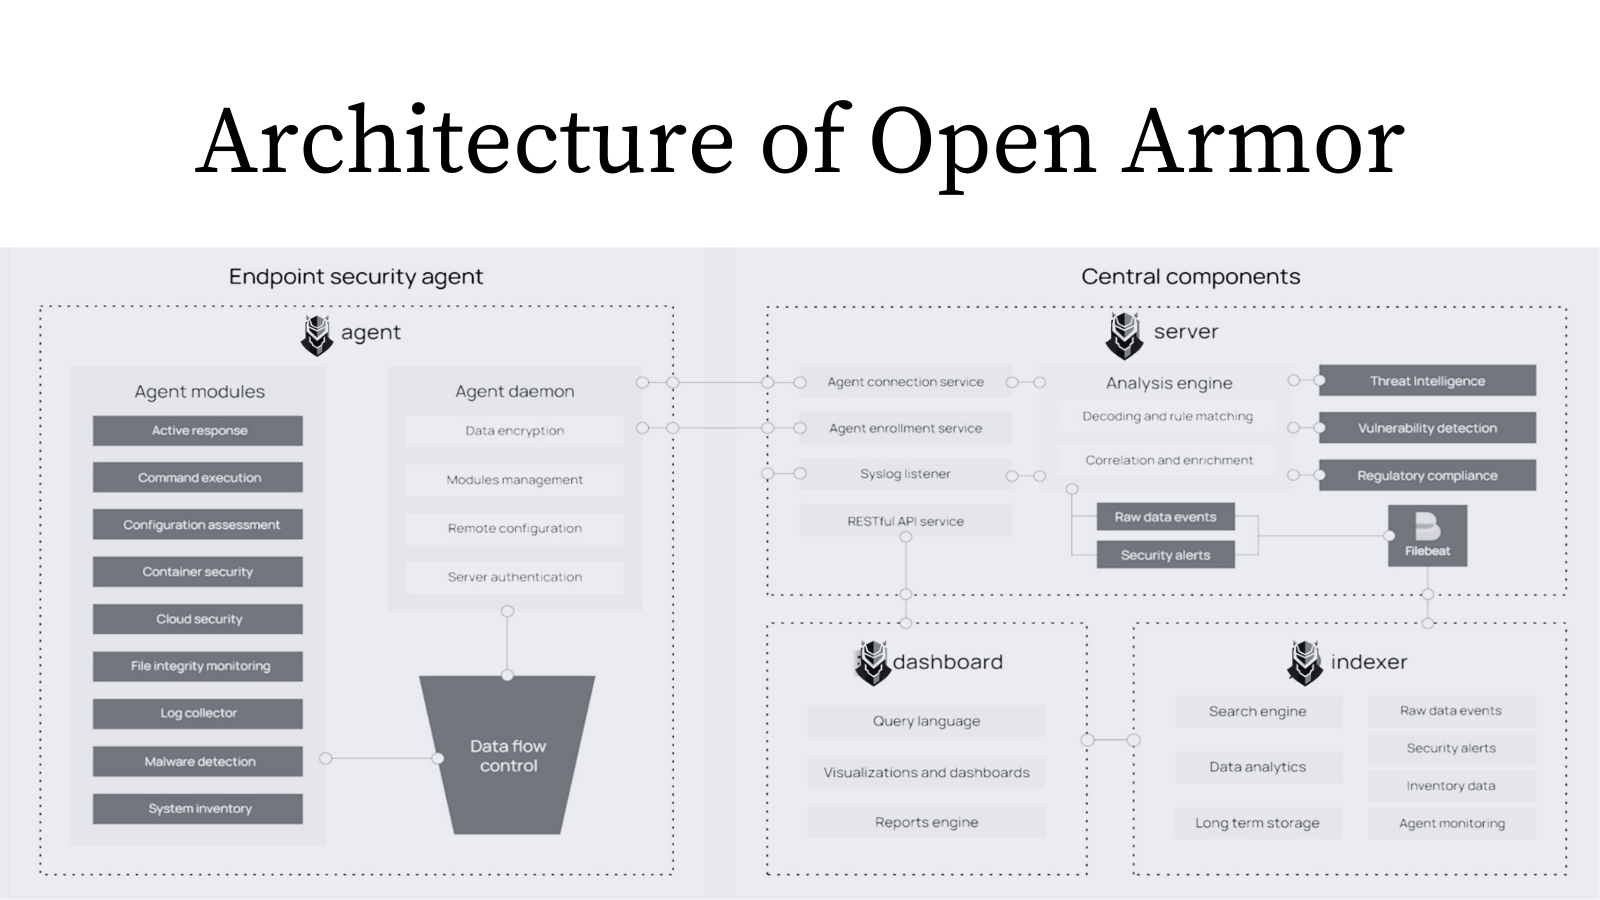
\includegraphics[width=1\linewidth]{OpenArmor_Architecture.png}
    \caption{OpenArmor High-Level Architecture}
    \label{fig:openarmor-architecture}
\end{figure}

\begin{figure}[h]
    \centering
    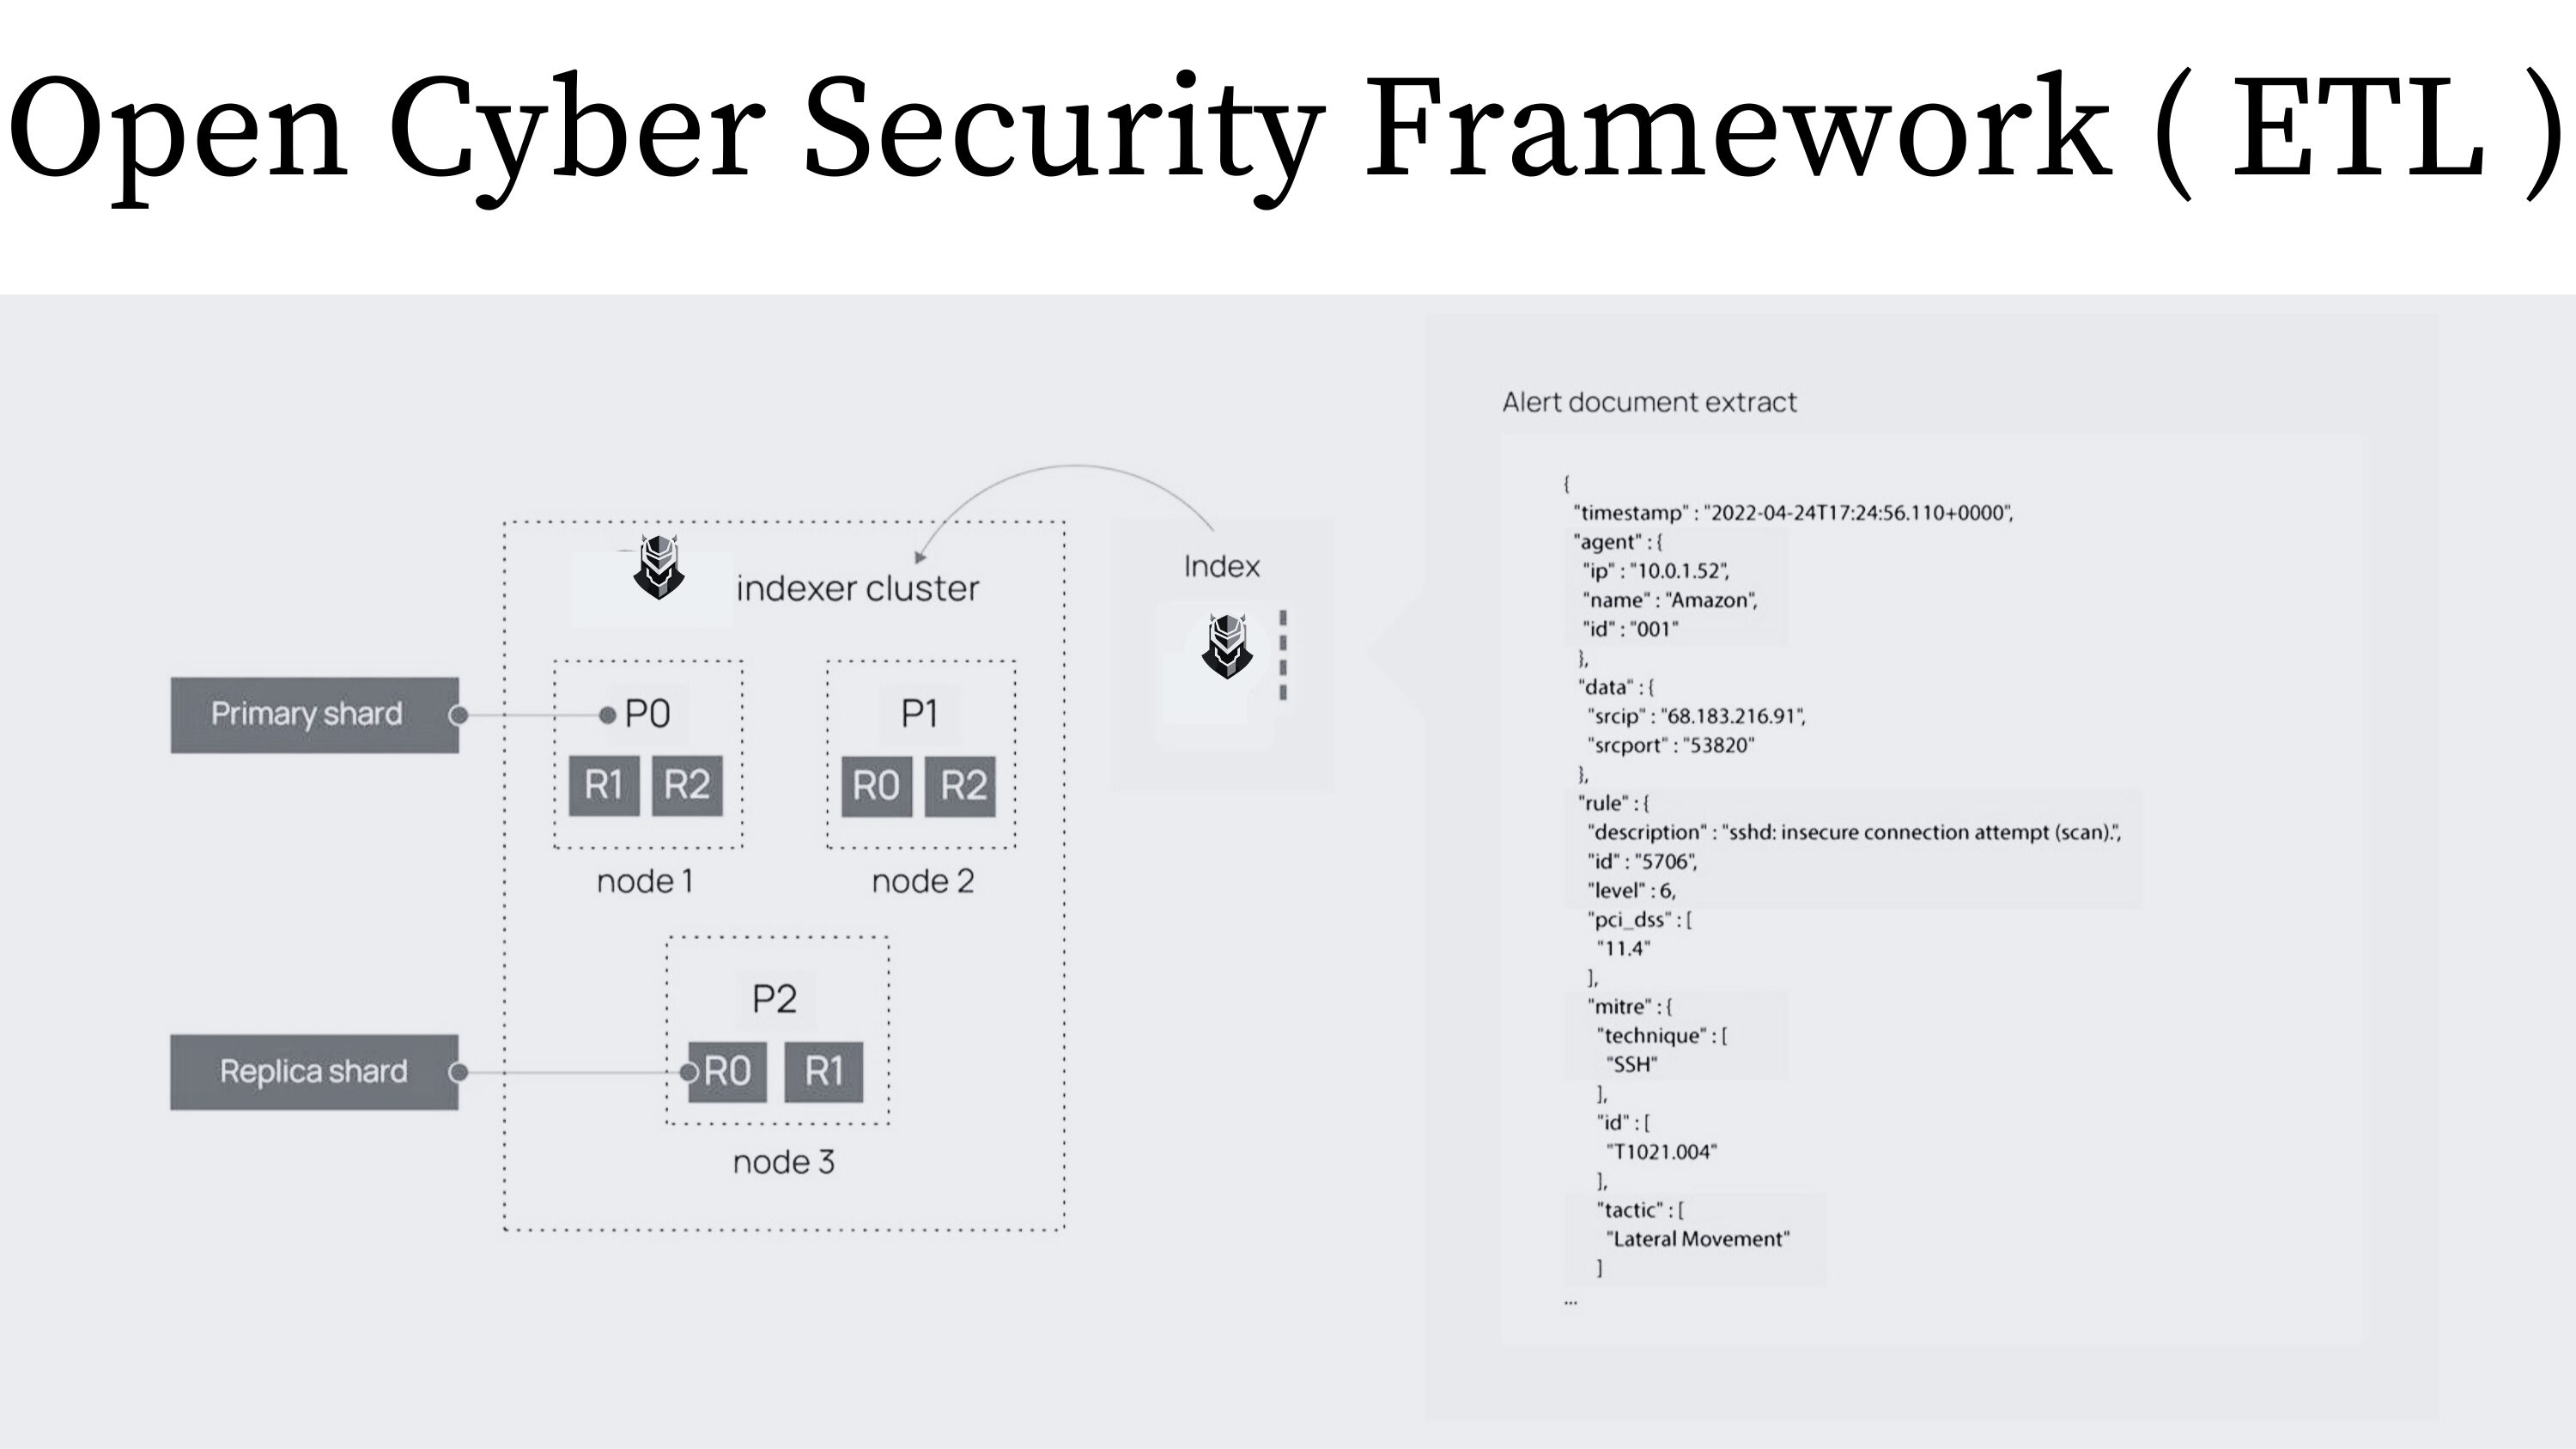
\includegraphics[width=1\linewidth]{ocsf-etl.png}
    \caption{OCSF Schema Parsing Architecture}
    \label{fig:ocsf-architecture}
\end{figure}

\begin{figure}[h]
    \centering
    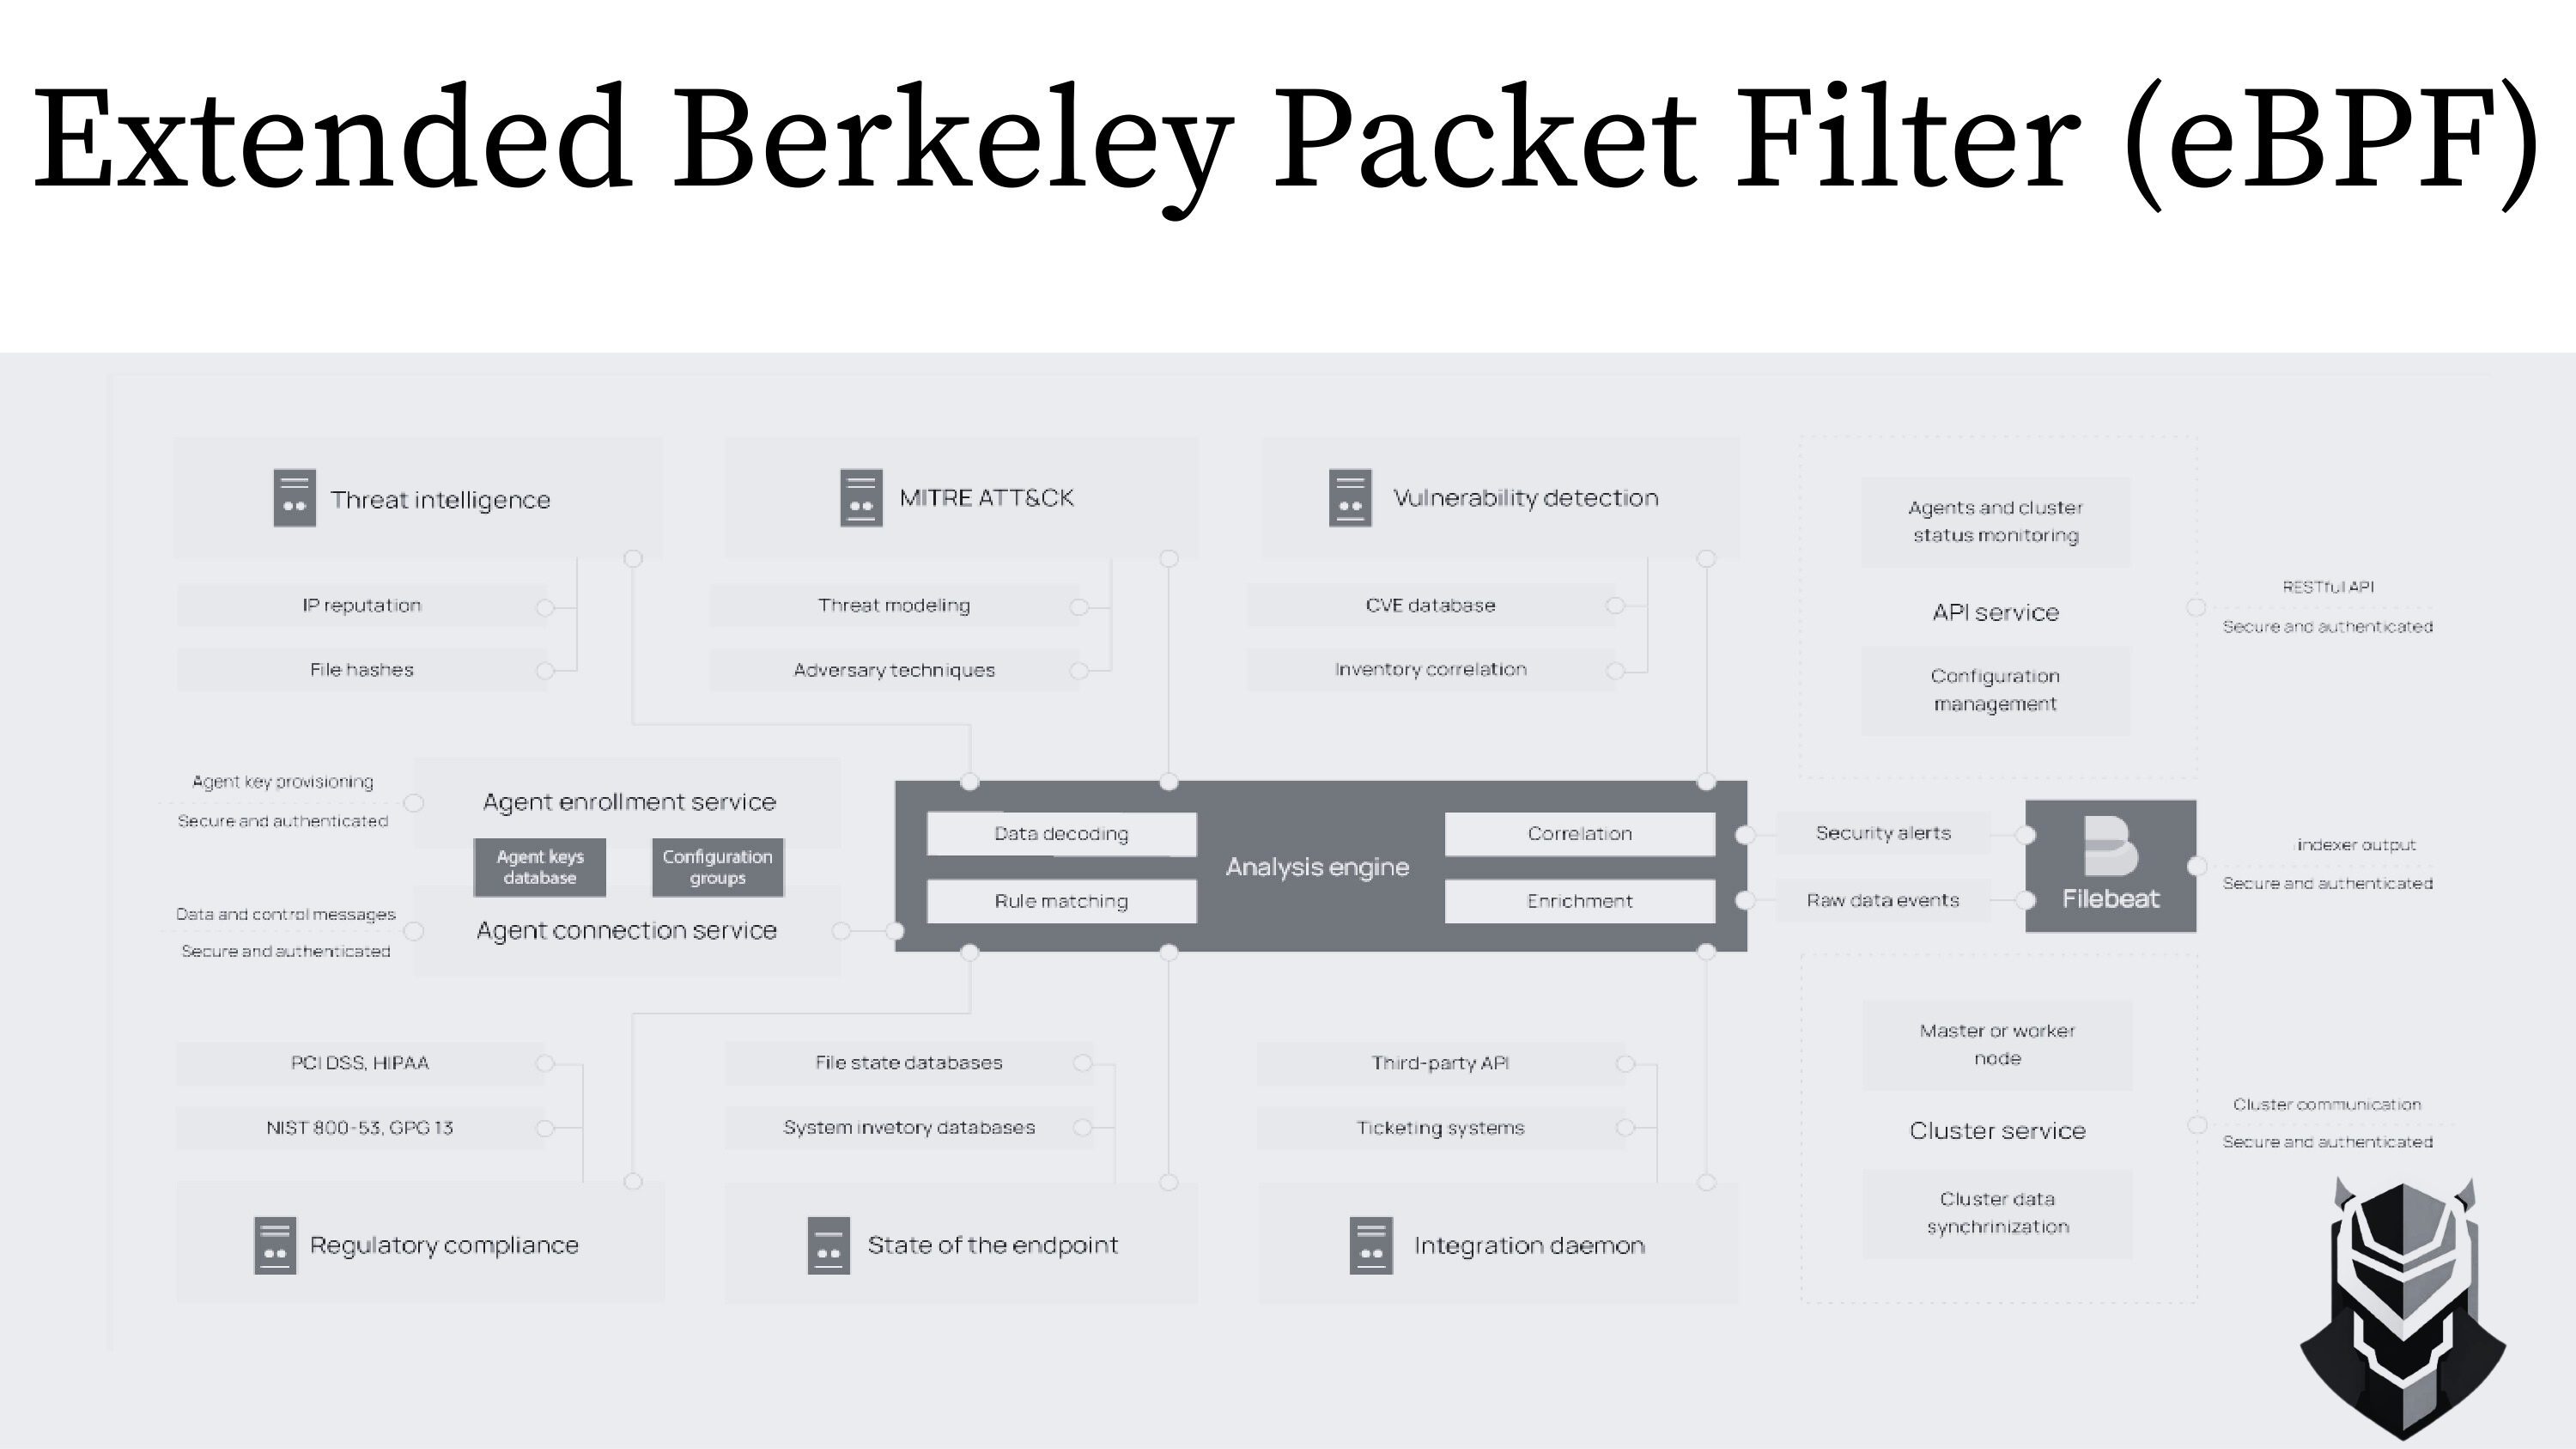
\includegraphics[width=1\linewidth]{ebpf-server.png}
    \caption{Extended Berkeley Packet Filter (eBPF) Server Side Architecture}
    \label{fig:ebpf-architecture}
\end{figure}

\begin{figure}[h]
    \centering
    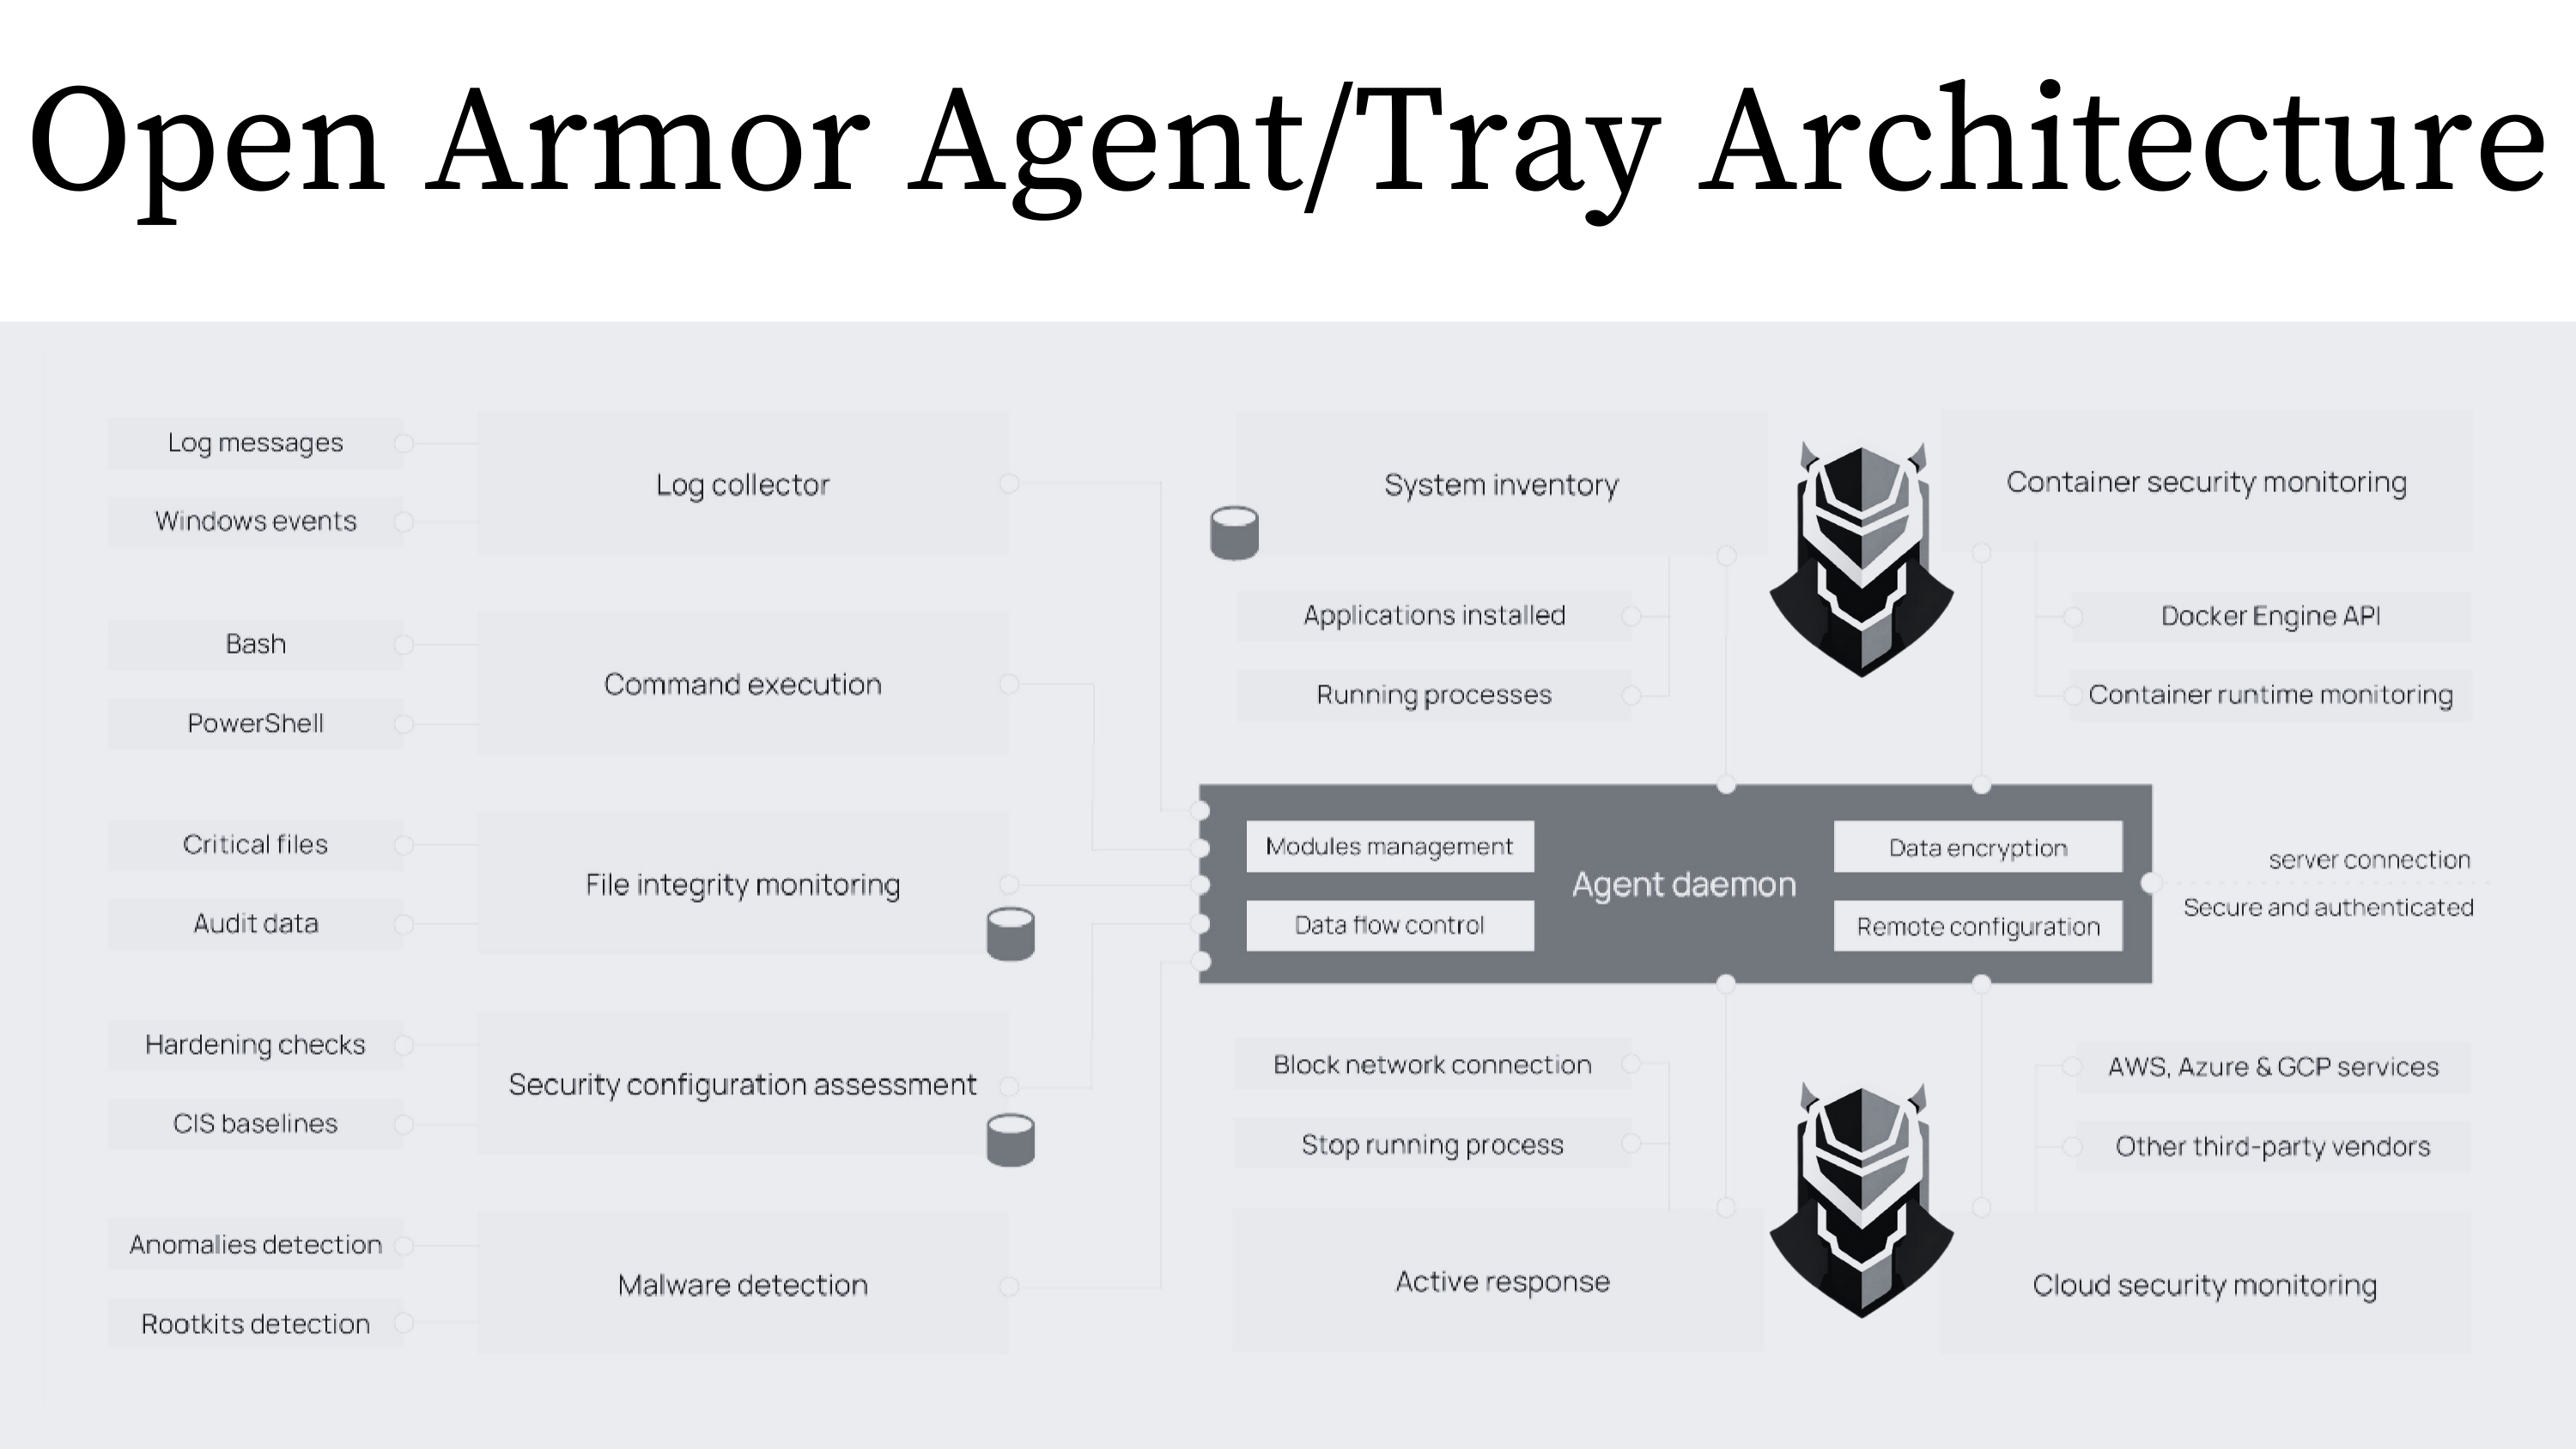
\includegraphics[width=1\linewidth]{openarmor-agent.png}
    \caption{Open Armor Agent Side Architecture}
    \label{fig:agent-architecture}
\end{figure}

\section{External Interfaces}

\subsection{User Interfaces}
OpenArmor's web-based dashboard serves as the primary user interface, incorporating:

\begin{itemize}
    \item Responsive design adhering to modern UI/UX principles
    \item Role-based access control for different user types
    \item Real-time event viewer with advanced filtering capabilities
    \item Customizable dashboards for various security metrics
    \item Interactive threat investigation tools
    \item Configuration management for agents and detection rules
\end{itemize}

\subsection{Hardware Interfaces}
OpenArmor interfaces with various hardware components, including:

\begin{itemize}
    \item Network Interface Cards (NICs) for packet capture and analysis
    \item Storage devices for log retention and database management
    \item Hardware Security Modules (HSMs) for secure key storage
    \item IPMI-enabled devices for out-of-band management in server environments
\end{itemize}

\subsection{Software Interfaces}
OpenArmor integrates with and extends several key software components:

\begin{itemize}
    \item Wazuh: Leveraging its HIDS capabilities and agent network
    \item OSquery: Utilizing its SQL-like interface for system state queries
    \item Sysmon: Incorporating its detailed Windows event logging
    \item SIEM Systems: Integration via OCSF-standardized logs
    \item Threat Intelligence Platforms: For IoC and threat data ingestion
\end{itemize}

APIs are provided for:
\begin{itemize}
    \item RESTful data access and management
    \item Webhook integrations for real-time alert notifications
    \item Custom plugin development and extension
\end{itemize}

\subsection{Communication Interfaces}
OpenArmor supports various communication protocols:

\begin{itemize}
    \item TLS-encrypted agent-server communication
    \item HTTPS for web interface access
    \item SSH for secure remote management
    \item Syslog for log ingestion from external sources
    \item MQTT for IoT device communication and monitoring
\end{itemize}

\section{System Features}

\subsection{eBPF-Enhanced Kernel Space Logging}
\subsubsection{Description and Priority}
High-priority feature for efficient, low-overhead kernel-level logging using eBPF technology.

\subsubsection{Stimulus/Response Sequences}
\begin{itemize}
    \item eBPF programs continuously monitor kernel events
    \item Relevant events are captured and streamed to the OpenArmor Core
    \item OpenArmor processes and correlates kernel-level data with other sources
\end{itemize}

\subsubsection{Functional Requirements}
\begin{itemize}
    \item REQ-1: Implement eBPF programs for comprehensive kernel event monitoring
    \item REQ-2: Develop a high-performance event streaming mechanism
    \item REQ-3: Create an extensible framework for custom eBPF programs
\end{itemize}

\subsection{OCSF Standardization and Integration}
\subsubsection{Description and Priority}
Critical feature for ensuring interoperability and standardized log formats across the system.

\subsubsection{Stimulus/Response Sequences}
\begin{itemize}
    \item Logs from various sources (Wazuh, OSquery, Sysmon, eBPF) are ingested
    \item OCSF Normalization Layer processes and standardizes the logs
    \item Standardized logs are made available for analysis and export
\end{itemize}

\subsubsection{Functional Requirements}
\begin{itemize}
    \item REQ-4: Develop adaptors for Wazuh, OSquery, and Sysmon log formats
    \item REQ-5: Implement OCSF schema mapping and validation
    \item REQ-6: Create an API for exporting OCSF-compliant logs to external systems
\end{itemize}

\subsection{AI-Driven Threat Detection}
\subsubsection{Description and Priority}
High-priority feature leveraging machine learning for advanced threat detection and analysis.

\subsubsection{Stimulus/Response Sequences}
\begin{itemize}
    \item AI Analytics Module continuously processes normalized log data
    \item Anomalies and potential threats are identified in real-time
    \item Alerts are generated and prioritized based on severity and confidence
    \item Threat intelligence is updated based on new findings
\end{itemize}

\subsubsection{Functional Requirements}
\begin{itemize}
    \item REQ-7: Develop and train ML models for anomaly detection
    \item REQ-8: Implement a real-time scoring system for threat prioritization
    \item REQ-9: Create an adaptive learning mechanism to improve detection over time
    \item REQ-10: Integrate with external threat intelligence sources for enhanced context
\end{itemize}

\subsection{Unified Query and Response System}
\subsubsection{Description and Priority}
Important feature providing a centralized interface for querying and responding to security events across all integrated components.

\subsubsection{Stimulus/Response Sequences}
\begin{itemize}
    \item User or automated system submits a query through the interface
    \item Query is distributed to relevant components (OSquery, Wazuh, eBPF engine)
    \item Results are collated, normalized, and presented to the user
    \item Automated response actions are suggested or executed based on query results
\end{itemize}

\subsubsection{Functional Requirements}
\begin{itemize}
    \item REQ-11: Develop a unified query language encompassing all data sources
    \item REQ-12: Implement query distribution and result aggregation mechanisms
    \item REQ-13: Create an automated response framework with customizable playbooks
    \item REQ-14: Provide an API for integrating the query system with external tools
\end{itemize}

\section{Data Design}
OpenArmor's data model is designed to efficiently store and process security events from various sources. Key components include:

\begin{itemize}
    \item Event Database: Stores normalized OCSF-compliant log entries
    \item Configuration Database: Manages system and agent configurations
    \item Threat Intelligence Database: Stores IoCs and threat patterns
    \item Machine Learning Model Storage: Retains trained ML models and their metadata
\end{itemize}

\section{Security and Privacy Design}
Security is paramount in OpenArmor's design, incorporating:

\begin{itemize}
    \item End-to-end encryption for all communications
    \item Secure key management using HSMs where available
    \item Role-based access control for all system functions
    \item Audit logging of all administrative actions
    \item Data anonymization techniques for privacy-sensitive information
    \item Regular security assessments and penetration testing
\end{itemize}

\section{Performance}
OpenArmor is designed to meet high-performance requirements:

\begin{itemize}
    \item Scalability to handle up to 100,000 endpoints in a single deployment
    \item Processing capability of up to 100,000 events per second
    \item Sub-second alert generation for critical threats
    \item Web interface response time under 2 seconds for most operations
    \item Efficient resource utilization on monitored systems (< 5% CPU, < 256MB RAM)
\end{itemize}

\section{Conclusion}
This system design outlines the architecture, interfaces, and key features of OpenArmor, integrating the strengths of Wazuh, OSquery, and Sysmon with innovative eBPF and AI-driven capabilities. The design emphasizes scalability, performance, and extensibility, positioning OpenArmor as a next-generation cybersecurity solution capable of addressing complex and evolving threat landscapes.